\documentclass{article}
\usepackage{ctex}
\usepackage{graphicx}
\usepackage{float}
\usepackage{geometry}
\usepackage{amssymb}
\usepackage{amsmath}
\usepackage{multirow}

%opening
\title{文泉考试平台 开发文档}
\author{200 OK}
\date{}
\geometry{a4paper, left=3.18cm, right=3.18cm, top=2.54cm, bottom=2.54cm}

\begin{document}

\maketitle

\section{需求分析}
    \subsection{用户管理}
        \begin{enumerate}
         \item 用户类型包括以下三种:超级管理员、管理员、学员
            \begin{itemize}
             \item 不同用户类型具有不同权限,同一页面显示内容应当根据用户权限改变。
            \end{itemize}
        \item 用户管理页面向管理员以列表形式呈现用户属性,包括用户名、类型、邮箱、最近登录IP
            \begin{itemize}
             \item 只有管理员可以进入用户管理页面;
             \item 其他用户尝试进入用户管理页面(如输入$url$)需有错误提示。
            \end{itemize}
        \item 管理员可创建、查看、编辑、封禁用户。
            \begin{itemize}
             \item 用户管理页面需添加按钮使管理员对用户进行创建、查看、编辑、封禁、解禁操作;
             \item 创建用户提供用户名、密码、邮箱、用户类型,且用户类型不能为超级管理员;
             \item 查看用户内容包括用户名、类型、邮箱、最近登录IP;
             \item 编辑用户内容包括将学生权限提升;
             \item 封禁用户后用户不能正常登录,并且在登录页面有错误提示;
             \item 管理员可以封禁学生,超级管理员可以封禁管理员,管理员不能封禁管理员。
            \end{itemize}
        \item 管理员由超级管理员创建,学员使用邮箱自行注册,通过邮箱激活。
            \begin{itemize}
             \item 超级管理员即$root$,只能伴随系统产生,只有一个,不能有其他途径创建;
             \item 管理员只能由超级管理员创建,或被从学生提升为管理员;
             \item 学员之间的区分以邮箱作为唯一标识,注册时需要对邮箱是否已注册进行检验;
             \item 学员成功注册后给相应邮箱发送邮件,包含导航至验证成功提示的页面的链接。
            \end{itemize}
        \end{enumerate}
        \begin{figure}[H]
            \centering
            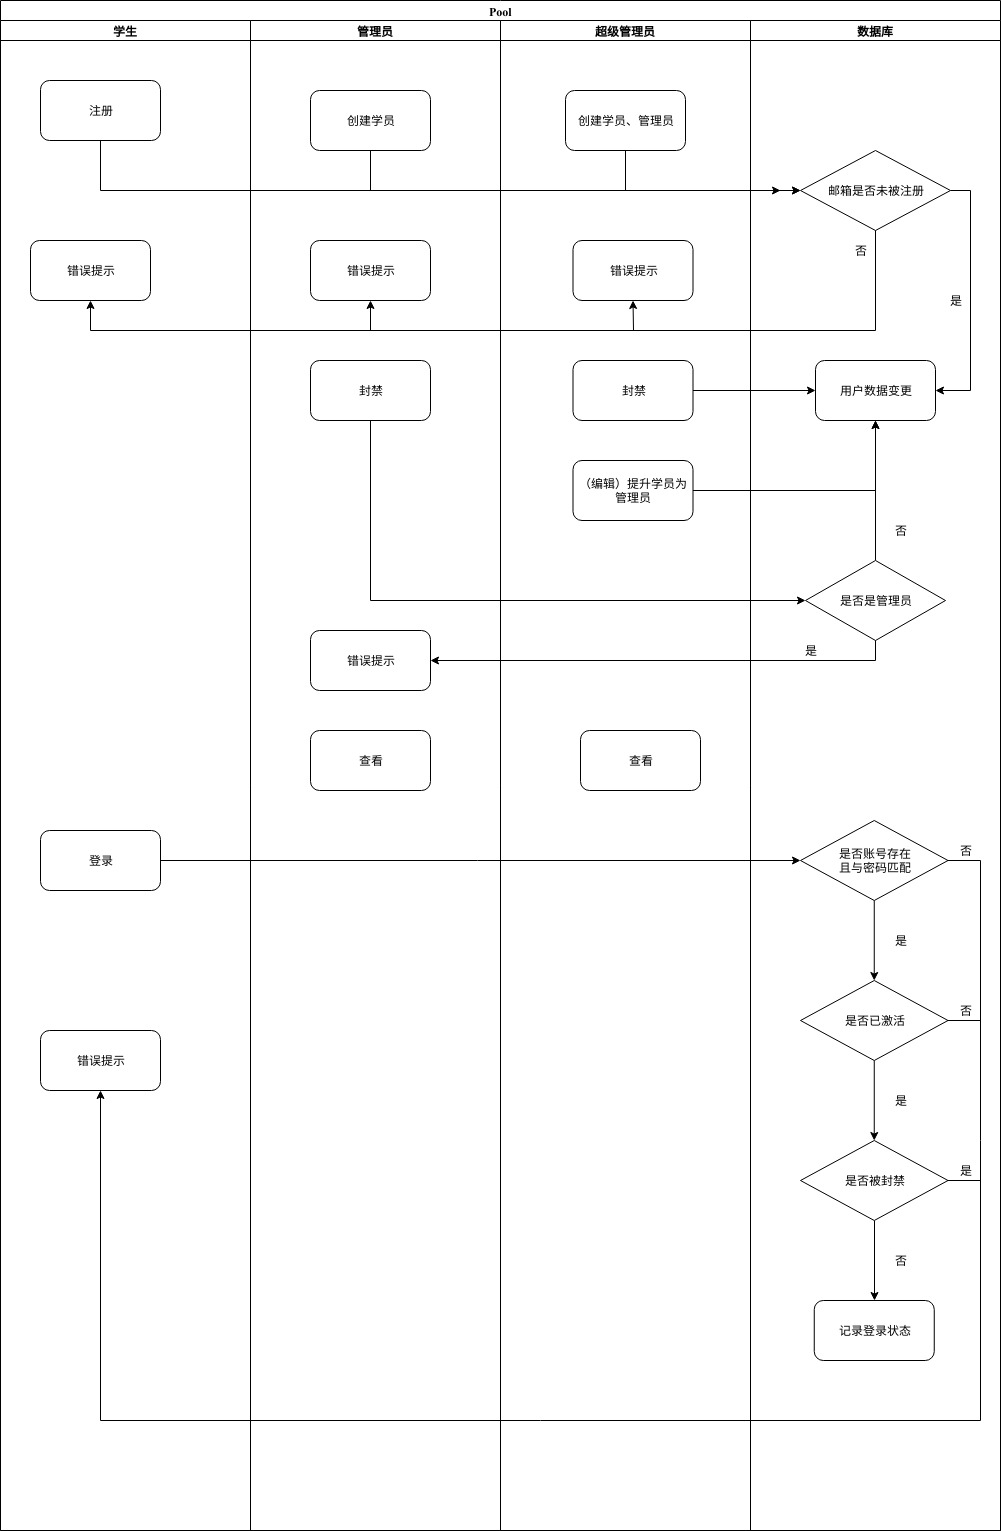
\includegraphics[width=.8\textwidth]{./UserManageMent.jpg}
        \end{figure}

    \subsection{题库管理}
    \begin{enumerate}
        \item 题库管理页面以列表的形式向管理员显示所有题库,包括题库名称、最后更新时间、题目数量。
        \begin{itemize}
            \item 题库管理有一个专门的页面;
            \item 题库管理界面默认为只读。
        \end{itemize}

        \item 管理员可以创建题库。
        \begin{itemize}
            \item 管理员在题库管理界面通过“创建”按钮进入“创建题库”,整个界面共用一个删除题库按钮;
            \item 创建题库的时候需要输入题库名称;
            \item 未输入题库名称时点击创建,不予以创建,并且弹出错误信息;
            \item 题库创建成功的时候转至被创建题库的界面;
        \end{itemize}

        \item 管理员可以编辑题库。
        \begin{itemize}
            \item 管理员在题库管理界面通过“修改”按钮开始修改题库,每个题库拥有一个“修改”按钮;
            \item 题库允许修改范围为题库名称;
            \item 修改完成以后需要点击“保存”按钮,保存成功时弹出成功信息;
            \item 若用户编辑以后未保存状态下离开界面,系统弹出提示信息,提示用户是否需要保存;若用户选择“是”,则保存并离开;若用户选择“否”,则不保存并离开;否则不保存并且不离开。
        \end{itemize}

        \item 管理员可以删除题库。
        \begin{itemize}
            \item 管理员在题库管理界面通过“删除”按钮进行删除题库,每个题库拥有一个“删除”按钮;
            \item 删除题库将删除题库中的所有题目;若题库中有题目被试卷组用,则不允许删除题库;
            \item 用户删除前,系统应该提示用户删除题库将造成的一系列后果,确认用户是否要删除该题库;若用户确认删除,则要求用户输入其密码以验证身份,身份确认之后再一次确认是否删除题库,若为是,则删除题库。
        \end{itemize}

    \end{enumerate}

    \subsubsection{习题}
    \begin{enumerate}
        \item 习题管理页面以列表的形式向管理员显示题库内的习题,包括类型、题面、题号、
        难度、更新时间。
        \begin{itemize}
            \item 习题管理界面有一个专门的页面,隶属于某个题库;
            \item 习题管理界面默认为只读。
        \end{itemize}

        \item 习题类型包括:单选题、多选题、判断题、填空题、问答题。其
        中,问答题为主观题,需要管理员进行评阅。习题属性还包括正确答案、题解,每个习题至少关联一个知识点。
        \begin{itemize}
            \item 单选题、多选题、判断题和填空题默认为系统自动批阅,管理员在批阅试卷的时候可以看到批阅结果,并对批阅结果进行修改。
        \end{itemize}

        \item 管理员可以对习题进行创建操作。
        \begin{itemize}
            \item 管理员通过点击“创建”按钮开始创建题目,整个页面共用一个创建按钮;
            \item 管理员需要选择题目类型,并且根据所选类型输入题目的题面、答案以及解析,并且为该题目选择一个知识点;
            \item 管理员需要点击“完成创建”按钮结束创建,若上述信息未输入,则不予以创建,并弹出错误信息;
            \item 创建成功时弹出成功信息。
        \end{itemize}

        \item 管理员可以对习题进行编辑操作。
        \begin{itemize}
            \item 管理员通过点击“编辑”按钮开始编辑题目,每个题目拥有一个修改按钮;
            \item 题库允许修改范围为题面、答案以及题解;
            \item 修改完成以后需要点击“保存”按钮,保存成功时弹出成功信息;
            \item 若用户编辑以后未保存状态下离开界面,系统弹出提示信息,提示用户是否需要保存;若用户选择“是”,则保存并离开;若用户选择“否”,则不保存并离开;否则不保存并且不离开。
        \end{itemize}

        \item 管理员可以对习题进行删除操作。
        \begin{itemize}
            \item 管理员通过点击“删除”按钮删除题目,每个题目拥有一个删除按钮;
            \item 若该题目被试卷组用,则拒绝删除;
            \item 删除之前要弹出对话框确认用户是否删除,若为是,则删除题目;否则不删除。
        \end{itemize}

    \end{enumerate}

    \subsubsection{知识点}
    \begin{enumerate}
        \item 知识点采用树形结构,管理员可以新建知识点树,拖动修改知识点级别。
        \begin{itemize}
            \item 知识点树显示在题库界面的指定UI区域中;
            \item 知识点树默认为只读;
            \item 管理员通过点击知识点树旁边的”修改“按钮,进入读写模式;
            \item 管理员点击知识点树上的创建按钮,创建叶子节点/子树,输入该节点的名称;若不输入,则用默认字符串填充;
            \item 管理员可以通过拖动修改知识点级别,例如将A子树拖到B子树下,则A子树成为B子树的子树;
            \item 修改完成以后需要点击“保存”按钮,保存成功时弹出成功信息;
            \item 若用户编辑以后为保存状态下离开界面,系统弹出提示信息;提示用户是否需要保存;若用户选择“是”,则保存并离开;若用户选择“否”,则不保存并离开;否则不保存并且不离开。
        \end{itemize}
    \end{enumerate}

    \subsubsection{试卷}
    \begin{enumerate}
        \item 试卷管理页面以列表的形式向管理员显示题库内的试卷信息,包括试卷名称、最后 更新时间、题目数量、总分数、状态(发布、草稿)。试卷还包含描述、限时的信 息。每份试卷由若干部分组成,每部分包含名称、题库内的若干习题,每道习题可 单独设置分数。
        \begin{itemize}
            \item 试卷管理有一个专门的页面,隶属于某一个题库。
            \item 试卷处于”草稿“状态的时候将只有管理员可见;处于”发布“状态的时候管理员、学员均可见,并且学员可以做题、提交。
        \end{itemize}

        \item 管理员可以对试卷进行创建操作。
        \begin{itemize}
            \item 管理员通过点击“创建”按钮进行创建试卷;
            \item 管理员需要设置试卷的若干个部分,每部分包含名称、题库内的若干习题,每道习题需要单独设置分数;
            \item 管理员需要设置试卷的描述以及限时;
            \item 管理员点击“完成创建”按钮完成创建,若上述要求输入的信息不符合要求,则不予以创建,并弹出错误信息;否则创建成功,被创建的试卷显示在试卷管理页面中,并且状态为“草稿”。
        \end{itemize}

        \item 管理员可以对试卷进行修改操作。
        \begin{itemize}
            \item 管理员可以点击”修改“按钮进行试卷修改;
            \item 管理员可修改范围同创建时要求输入的内容;
            \item 修改完成后点击“保存”按钮进行保存;如果修改后的信息不符合要求,则不允许保存,并报出错误信息;
            \item 若用户编辑以后为保存状态下离开界面,系统弹出提示信息;提示用户是否需要保存;若用户选择“是”,则保存并离开;若用户选择“否”,则不保存并离开;否则不保存并且不离开。
        \end{itemize}

        \item 管理员可以对试卷进行查看操作。
        \begin{itemize}
            \item 管理员可以通过点击“查看”按钮查看试卷的具体信息。
        \end{itemize}
        \item 试卷批阅页面以列表的形式向管理员显示题库内所有学员提交的试卷,包括试卷名 称、提交时间、学员名称。管理员可对试卷给出评分、做出评语。
        \begin{itemize}
            \item 试卷管理页面有一个专门的页面,隶属于某一个题库;
            \item 当学员提交试卷以后,该试卷将在试卷批阅页面中显示;
            \item 客观题将由系统根据答案进行批阅,主观题由管理员批阅;管理员也可以查看并修改系统的批阅结果;
            \item 主观题需要手动赋分;
            \item 管理员完成批阅后,批阅结果将被推送给学员。
        \end{itemize}
    \end{enumerate}

    \subsubsection{权限码}
    \begin{enumerate}
        \item 权限码用于赋予学员使用题库内习题和试卷的权限。
        \begin{itemize}
            \item 学员在指定区域输入权限码来激活题库,学员只能访问被激活题库下的题目和试卷。
        \end{itemize}

        \item 权限码管理页面以列表形式向管理员显示题库的权限码信息,包括总数、未激活数量、已激活数量、生成时间。
        \begin{itemize}
            \item 权限码管理有一个专门的界面,隶属于某一个题库;
            \item 该界面显示当前题库的权限码信息。
        \end{itemize}

        \item 管理员可以进行生成权限码。权限码是由数字和字母组成的唯一值。
        \begin{itemize}
            \item 管理员通过点击权限码管理界面上的“生成权限码”按钮生成权限码;
            \item 管理员需要输入生成权限码的数量。
        \end{itemize}

    \end{enumerate}
    
    \subsection{学习系统}
    	\begin{enumerate}
    		\item 在登陆之后,学生可以选择题库开始学习。
    		\item 学习系统分为两个板块:自主练习、试卷模考。
    		\item 进入自主练习模块后,学生可以选择知识点练习该题库下的题目。
    		\begin{itemize}
    			\item 学生需要先选择题库后才能继续;
    			\item 输入习题数量之后,系统从题库中抽取对应数量的题目,然后开始练习;
    			\item 答题完毕后显示答案对错与题目解析;
    			\item 题目抽取时不抽取主观题。
    		\end{itemize}
   			\item 进入试卷模考模块后,学生可以完成后台试卷管理创建的试卷。
   			\begin{itemize}
   				\item 试卷完成后系统批阅客观题,主观题提交到后台等待批阅;
   				\item 试卷完成后直接显示客观题批阅结果;
   				\item 试卷批阅完成后在查看试卷时显示评分和批语。
   			\end{itemize}
    	\end{enumerate}
    \subsection{非功能需求}
		\begin{enumerate}
			\item 平台界面设计合理、逻辑清晰。
			\item 平台能兼容电脑、手机和平板等终端浏览器浏览。
			\item 对用户易于学习和使用,用户体验友好。
			\item 根据用户权限控制访问数据,进行操作记录。
			\item 系统出错时,不影响用户的行为操作与数据。
		\end{enumerate}
		
\section{模块及接口}
    \subsection{前端}
    	
    	\paragraph{QuestionShow}
    		\subparagraph{描述}
                显示习题题干、学生回答、标准回答、分数、阅卷者评论等内容的基类
            \subparagraph{调用} RichTextEditor
    		\subparagraph{属性} \ \par
                \subitem{id:习题对应的唯一id}
       
       \paragraph{QuestionSingleChoice}
            \subparagraph{描述}
                创建和修改单选题目信息的组件
            \subparagraph{调用} RichTextEditor
            \subparagraph{属性} \ \par
                \subitem{readonly:是否只读} \par
                \subitem{TF:是否是判断题} \par
                \subitem{creation:是否是在创建题目}\par
        \paragraph{QuestionSolve}
            \subparagraph{描述}
                学员答题组件
            \subparagraph{调用}
                QuestionShow
            \subparagraph{属性} \ \par
                \subitem{answer:传入的学员答案}\par
                \subitem{id:习题的唯一标识符id}\par
                \subitem{readonly:是否只读}\par
       
       \paragraph{RichTextEditor} \ \par
            \subparagraph{描述}
                富文本编辑器,使用markdown格式存储
            \subparagraph{调用} ImageUploader
            \subparagraph{属性} \ \par
                \subitem{readonly:是否只读}\par
                \subitem{placeholder:空白时的占位文字}\par
                \subitem{label:文本框标签}\par
                \subitem{content:文本内容} \par
                \subitem{required:是否为必填项}
                
        \paragraph{SignInBox}
            \subparagraph{描述}
                用户登录时填账号密码的区域
          
        \paragraph{SignUpBox}
            \subparagraph{描述}
                用户注册时填充信息的区域
        
        \paragraph{TestPaper}
            \subparagraph{描述}
                试卷修改与创建的组件
            \subparagraph{调用}
                QuestionBanksList, QuestionList, QuestionListItem
            \subparagraph{属性}\ \par
                \subitem{paper:传入的试卷数据}
                \subitem{id:试卷的唯一标识符id}
                \subitem{editable:是否正在进行修改}
                \subitem{create:是否正在创建卷子}
                
        \paragraph{TestPaperMarkingList}
            \subparagraph{描述}
                查看所有需要批改的试卷的列表
            \subparagraph{调用}
                TestPaperMarkingListItem
            \subparagraph{属性}\ \par
                \subitem{title:列表的标题}
                
        \paragraph{TestPaperMarkingListItem}
            \subparagraph{描述}
                需要批阅的试卷的列表中的单个项目
            \subparagraph{属性}\ \par
                \subitem{id:试卷记录的唯一标识符id}
                \subitem{readonly:是否只读}
                
        \paragraph{TestPaperRecordList}
            \subparagraph{描述}
                学员端看到的自己所做的所有试卷的历史记录列表
            \subparagraph{调用}
                TestPaperMarkingListItem
            \subparagraph{属性}\ \par
                \subitem{title:列表的标题}
                
        \paragraph{TestPapersList}
            \subparagraph{描述}
                所有可以做的试卷的列表
            \subparagraph{调用}
                TestPaper, TestPapersListItem
            \subparagraph{属性}\ \par
                \subitem{title:列表的标题}
                \subitem{readonly:是否只读}
                
        \paragraph{TestPapersListItem}
            \subparagraph{描述}
                可以做的试卷的列表中的单个项目
            \subparagraph{属性}\ \par
                \subitem{test\_paper:传入的试卷信息}
                \subitem{readonly:是否只读}
            
        \paragraph{TreeView}
            \subparagraph{描述}
                知识树结构
            \subparagraph{属性}\ \par
                \subitem{editable:是否正在修改}
                \subitem{selection:选中的节点}
                \subitem{rootID:根节点的唯一标识符id}
                
        \paragraph{UserTable}
            \subparagraph{描述}
                查看用户信息的列表
            \subparagraph{属性}\ \par
                \subitem{users:用户信息的数组}
                
        \paragraph{WrongQuestionsCollection}
            \subparagraph{描述}
                错题集
            \subparagraph{调用}
                QuestionCorrect
    \subsection{后端}
    
\section{数据库设计}

\end{document}
